\documentclass[tikz,border=6pt]{standalone}
\usepackage[T1]{fontenc}
\usepackage[utf8]{inputenc}
\usepackage{helvet}
\renewcommand{\familydefault}{\sfdefault}
\usetikzlibrary{positioning}

\begin{document}
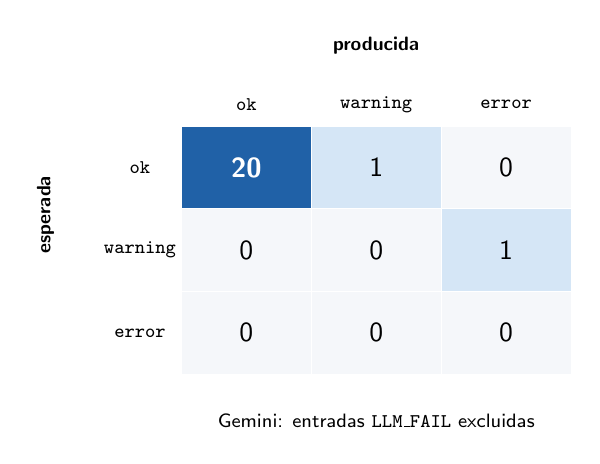
\begin{tikzpicture}[
    font=\sffamily,
    cell/.style={rectangle, draw=white, minimum width=1.65cm, minimum height=1.05cm, align=center},
    head/.style={font=\sffamily\scriptsize\bfseries, align=center},
    axis/.style={font=\sffamily\scriptsize, align=center}
]
\definecolor{c0}{RGB}{245,247,250}
\definecolor{c1}{RGB}{213,230,246}
\definecolor{c2}{RGB}{160,202,234}
\definecolor{c3}{RGB}{32,97,167}

\node[head] at (2.55, 3.2) {producida};
\node[head, rotate=90] at (-1.65, 1.05) {esperada};
\node[axis] at (0.9, 2.45) {\texttt{ok}};
\node[axis] at (2.55, 2.45) {\texttt{warning}};
\node[axis] at (4.2, 2.45) {\texttt{error}};
\node[axis] at (-0.45, 1.65) {\texttt{ok}};
\node[axis] at (-0.45, 0.6) {\texttt{warning}};
\node[axis] at (-0.45, -0.45) {\texttt{error}};

\node[cell, fill=c3, text=white, font=\sffamily\bfseries] at (0.9, 1.65) {20};
\node[cell, fill=c1] at (2.55, 1.65) {1};
\node[cell, fill=c0] at (4.2, 1.65) {0};
\node[cell, fill=c0] at (0.9, 0.6) {0};
\node[cell, fill=c0] at (2.55, 0.6) {0};
\node[cell, fill=c1] at (4.2, 0.6) {1};
\node[cell, fill=c0] at (0.9, -0.45) {0};
\node[cell, fill=c0] at (2.55, -0.45) {0};
\node[cell, fill=c0] at (4.2, -0.45) {0};

\node[axis, below=0.35cm] at (2.55, -1.0) {Gemini: entradas \texttt{LLM\_FAIL} excluidas};
\end{tikzpicture}
\end{document}
